
\lettrine{A}{ccording} to research by First Education (2022), the Dutch are positioned as the most proficient English-speaking population globally. Other countries that achieved a position in the top 10 ranking were Denmark, Belgium, Sweden, Finland, and Germany. While a proud Dutchman may attribute this success to hard work and dedication, it is worth considering other factors that could be at play here. Notably, these countries with commendable English proficiency are all located in North Europe and speak very similar languages.  

Linguistics offers a unique perspective on the relationships between different languages. By comparing the vocabulary, grammar and sound systems of various languages, researchers have identified related language families and have constructed language family trees to illustrate the evolution and divergence of languages over time. Thanks to that research, we know that many countries with notable position in the English Proficiency Index share a common linguistic background. Such a linguistic background, or language family, thus may provide a foundation for proficiency in a new language. 

This would imply that certain languages are easier to learn for certain population groups. For Atlan, it is deemed important that it will become a language that is easy and quick to learn for \textit{everybody}. This is a challenging task but might be achievable if we find some sort of shared background between almost every natural language. If it is possible to find words that look similar in different languages, which are known as cognates, the translation for those words in Atlan can be designed to resemble them as much as possible. With a model that can do this on a large scale, Atlan will become easy, neutral, and global.  

To achieve this, it is first key to create some understandings of what methods are used to compare different languages. Therefore, we will take a closer look at the so-called cosine similarity. Thereafter, it is necessary to conduct an examination of the existing language families that exist. In that way, we gain a deeper insight into the connections between existing natural languages. In addition, with that gained understanding, it is possible to decide which language we will make available in contributing to the process of cognate finding. The most spoken languages are weighed against each other to create a dataset that is representative of the real world. All these pieces of the puzzle come together in the final part of this chapter, where the computer program that we used to generate words in Atlan will be discussed.

\section{Comparison methods and language families}

\subsection{Cosine Similarity}

According to research by First Education (2022), the Dutch are positioned as the most proficient English-speaking population globally. Other countries that achieved a position in the top 10 ranking were Denmark, Belgium, Sweden, Finland, and Germany. While a proud Dutchman may attribute this success to hard work and dedication, it is worth considering other factors that could be at play here. Notably, these countries with commendable English proficiency are all located in North Europe and speak very similar languages.  

Linguistics offers a unique perspective on the relationships between different languages. By comparing the vocabulary, grammar and sound systems of various languages, researchers have identified related language families and have constructed language family trees to illustrate the evolution and divergence of languages over time. Thanks to that research, we know that many countries with notable position in the English Proficiency Index share a common linguistic background. Such a linguistic background, or language family, thus may provide a foundation for proficiency in a new language. 

This would imply that certain languages are easier to learn for certain population groups. For Atlan, it is deemed important that it will become a language that is easy and quick to learn for \textit{everybody}. This is a challenging task but might be achievable if we find some sort of shared background between almost every natural language. If it is possible to find words that look similar in different languages, which are known as cognates, the translation for those words in Atlan can be designed to resemble them as much as possible. With a model that can do this on a large scale, Atlan will become easy, neutral, and global.  

To achieve this, it is first key to create some understandings of what methods are used to compare different languages. Therefore, we will take a closer look at the so-called cosine similarity. Thereafter, it is necessary to conduct an examination of the existing language families that exist. In that way, we gain a deeper insight into the connections between existing natural languages. In addition, with that gained understanding, it is possible to decide which language we will make available in contributing to the process of cognate finding. The most spoken languages are weighed against each other to create a dataset that is representative of the real world. All these pieces of the puzzle come together in the final part of this chapter, where the computer program that we used to generate words in Atlan will be discussed.
\vspace{0.3cm}

\begin{center}
\resizebox{1\textwidth}{!}{
\begin{tabular}{|c|c|c|}
\hline
{\bf Text} & {\bf Frequency \lq\lq Merry"} & {\bf Frequency \lq\lq christmas"} \\
\hline

\lq\lq Merry christmas " & 1 & 1 \\

\lq\lq Christmas" & 0 & 1 \\
\hline
\end{tabular}
	}

{\it \footnotesize Table 6.1: Word-appearance in \lq\lq Merry" and \lq\lq Merry christmas".}
\end{center}
\vspace{0.3cm}

 \noindent This table can be visualized in a two-dimensional array, where on each axis the count of a word is represented. Now both texts can be placed as a dot on this grid accordingly. Drawing two lines from each point to the origin of the grid creates an angle between those lines. This angle at the origin can be calculated, in this case it would be 45$^{\circ}$ . To finish the cosine similarity, all that is needed now is to take the cosine of this angle, in this example \textit{cos (45)} = 0.71. 


\begin{center}
	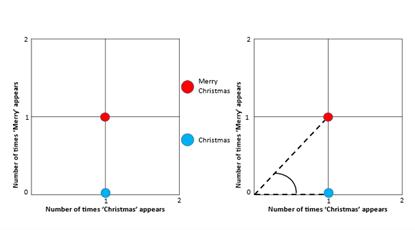
\includegraphics[scale=0.8]{./Images/graphs.jpg}
	{\it \footnotesize Figure 6.1: Graph depicting word-appearance}
\end{center}

If the compared sentences are identical, the two dots would be placed on the same place in the grid. Thus, the lines towards the origin would fall precisely over each other. Therefore, the angle between both lines would be 0$^{\circ}$, resulting in a cosine score of \textit{cos (0) = 1.} On the other hand, if both sentences have not a single element in common, the lines would be perpendicular to each other. With an angle of 90$^{\circ}$, the cosine similarity would return \textit{cos (90) = 0.} Thus, in any case, the cosine similarity gives a score between 0 and 1, showing the degree of similarity. 

As another example, let’s compare two words: \textit{‘Bert’} to \textit{‘Ernie’}. Instead of words, the vector now can be made up of letters. In a table, this would look like this:

\begin{center}
\begin{tabular}{|l|c|c|c|c|c|c|c|}
\hline
{\bf Name} & {\bf E} & {\bf R} & {\bf N} & {\bf I} & {\bf B} & {\bf T} \\
\hline
{\bf Ernie} & 2 & 1 & 1 & 1 & 0 & 0\\
{\bf Bert} & 1 & 1 & 0 & 0  & 1 & 1 \\
\hline
\end{tabular}

{\it \footnotesize Table 6.2: Letter frequency in the words \lq\lq Bert" and \lq\lq Ernie".}
\end{center}

\noindent With six different letters occurring, it would be possible to place both \textit{‘Bert’} and \textit{‘Ernie’} in a six-dimensional grid and draw the lines to the origin. However, it is impossible for humans to visualize a six-dimensional graph. Thus, we need a new way to calculate the angle between the two vectors. Luckily, there exists a formula to compute the cosine similarity. 

\begin{center}
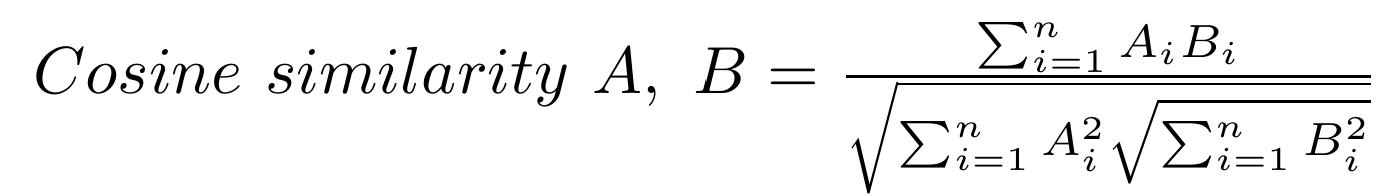
\includegraphics[scale=0.2]{./Images/cosine.jpeg}
\end{center}

%\begin{center}
%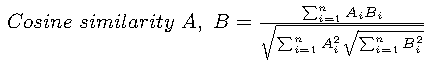
\includepdf[scale=0.5]{./Mainmatter/sum.pdf}
%\end{center}
%\end{samepage}

%\begin{equation}
%Cosine~ similarity~ A, ~B = \frac{\sum_{i=1}^{n} A_i B_i}{\sqrt{\sum_{i=1}^{n} A_i^2 \sqrt{\sum_{i=1}^{n} B_i^2}}}
%\end{equation}

In less mathematical terms, what this means is that each element of the two vectors A and B are compared. The products of all the elements are then summed up and divided by the length of both the vectors together. If we fill in the numbers for our Bert-Ernie-comparison, it will look like this: 

%\resizebox{1\textwidth}{!}{
{\small
%\begin{equation}
	\[
	\frac{1 \times 2 + 1 \times 1 + 1 \times 0 + 1 \times 0 + 0 \times 1 + 1 \times 0}{\sqrt{2^2 + 1^2 + 1^2 + 1^2 + 0^2 + 0^2 \sqrt{1^2 + 1^2 + 0^2 + 0^2 + 1^2 + 1^2}}} = 0.56
\]
%\end{equation}
%}
}

Nevertheless, converting the words based solely on letter frequency inadvertently results in losing vital information about the arrangement of the letters. This preservation is of utmost importance for our project since we try to find patterns and therefore adjacent letter combinations. To address this concern, we introduced a slight adjustment to the regular cosine similarity, where each index with the same character in both words also scores a small point. In this way, our cosine similarity tries to reward words that have the same letters on the same place.

\subsection{Language families}

The use of various comparison methods, similar to the cosine similarity, allowed linguists to identify several groups of related languages. These groups, or language families, were categorized based on common linguistic features and a shared common ancestor (Campbell, 2018). Such a common Proto-Language allows researchers to trace origins of various languages to a single root. However, this does not necessarily need to be the case. There exist languages for which it is impossible to classify them as part of a language family, such as Basque (Campbell, 2010). Researchers speculate that it might be possible that these languages, known as language isolates, might have had related languages in the past, that went instinct unrecorded. Therefore, these languages now form their own language family, with them being the only member. On the other hand, not only genetic proximity between languages is enough to be placed in the same language family. Languages that are constructed instead of naturally developed cannot be considered part of any language family, since they do not have a shared ancestor with any other language (Campbell, 2018). 

Although this means that the total number of language families in the world might be in the hundreds, not all are equally relevant today. To begin with, 94 language families are extinct, meaning there is a lack of any surviving speakers (Campbell, 2018). In addition, the number of languages and the number of speakers differ largely. There are five language families that can be considered as the main language families of the world. Every single one of these languages contains at least 5% of the languages in the world and combined they capture more than two-thirds of all the natural languages. The families are called Indo-European, Sino-Tibetan, Niger-Congo, Austronesian and Afro-Asiatic.  

The most widely spoken language family, with over 3 billion speakers worldwide today, is Indo-European. When Sir William Jones first spoke of this family, he proposed there were several branches with related languages (Fortson, 2011). First, there is \textit{Indo-Iranian}, spoken in the middle east, where the languages Sanskrit, Persian and Pashto are placed. Secondly, \textit{Italic}, with languages such as Latin, Italian and Spanish. Third, the languages of the Northern parts of Europe were placed in the \textit{Germanic} branch. A fourth branch called \textit{Celtic} housed the languages of the island of Great Britain, such as Irish and Welsh. Lastly, Jones portrayed one branch on its own for \textit{Greek}.. Only after thirty years would this division be altered, when researchers added three more branches to the family. The largest new branch was called the \textit{Balto-Slavic} branch, including languages such as Russian, Ukrainian and Czech. The two remaining branches both only contained one language, \textit{Armenian} and \textit{Albanian.} This family tree remained the same to this day, except for the addition of two branches with extinct languages discovered in the first half of the 20th century, called \textit{Anatolian} and \textit{Tocharian.}  

The Sino-Tibetan language family is, even though it has more daughter languages than Indo-European, the second most spoken family, with around 1.3 billion speakers. This family can be split up into two major subgroups: \textit{Chinese} and \textit{Tibeto-Burman}  (Shafer, 1955). The Chinese subgroup is like a family on its own, made up of different but related dialects. The largest and best-known ones are Mandarin and Cantonese. Tibeto-Burman can be branched into a few branches on its own: Tibetic (Tibetan), Burmese-Lolo (Burmese and various Lolo-languages) and Karenic.  

Niger-Congo is the third most spoken family, containing the highest number of languages: over 1,500 languages are known ancestors of the Proto-Niger-Congo language. Although this number is nearly twice that of Indo-European, it is spoken by 600 million people, due to the immense language diversity in the Sub-Saharan Africa region (Heine et al., 2000). The largest branch in the Niger-Congo family is called the \textit{Atlantic-Congo} branch. Herein are numerous languages spoken in West Africa, such as Yoruba and Igbo. Also, Swahili, mostly spoken in the Eastern part of Africa, falls into this category. The languages spoken in the Central and Southern parts of Africa are mostly from another branch, called the \textit{Bantu-Congo} branch. These are languages such as Zulu, Xhosa and Shona. Other branches are the \textit{Kordofanian} branch (Katla, Moro and Talodi) and \textit{Mande} branch (Bambara, Mandinka and Soninke) 

Austronesian, with a similar high diversity as Niger-Congo, covers the languages found in the region that stretches from Southeast-Asia to the Pacific Island. In total this family contains more than 1,200 languages and is spoken by approximately 326 million speakers, primarily in countries such as Indonesia, Malaysia and the Philippines. The most important subgroup within this family is the \textit{Formosan} branch, forming a total of nine distinct branches (Tryon, 1995). These branches are all made up of the different indigenous languages of Taiwan. None of them are, however, the most widespread or diverse branch of the family. This is namely the tenth branch, known as the \textit{Malayo-Polynesian} branch, encompassing Indonesian, Javanese and Sundanese.  

Lastly, the languages mostly spoken in the North and the Horn of Africa and Southwest Asia are grouped in the Afroasiatic language family.  This family consists of several branches (Huernergard, 2004). The one that houses the best-known languages is the \textit{Semitic} branch, including Arabic, Amharic and Hebrew. Another large branch is \textit{Berber}, with languages such as Tamazight and Kabyle. Smaller branches are the \textit{Cushitic} branch, which comprises of languages such as Oromo, Somali and Afar, and the \textit{Chadic} branch, with as largest language Hausa. The languages in the Afroasiatic family combined are spoken worldwide by almost 600 million people. 


\section{Using cognates to generate words}


A study by Otwinowska and Szewczyk (2018) argued that cognates, similar sounding words with the same meaning in different languages, are the easiest words to learn when learning a new language. The resemblance with your mother tongue makes the words much easier to remember and use then non-cognates words. By designing Atlan in a way that it has a lot of these cognates, we try to keep the trouble of learning Atlan as low as possible. To achieve this goal, it is key to make new Atlan words resemble existing words, or patterns in existing words, as much as possible. 

The idea of using cognates to generate new words for vocabulary is also used in the creation of the constructed language Lojban (Cowan, 1997).  Lojban proposed new words, or ‘gismu’s’ and looked for words that looked similar to it in the languages Chinese, English, Spanish, Hindi, Russian and Arabic. If three or more letters were the same and in the same order as a word in the source language, the gismu would score points. For resemblance with larger language a gismu could score more points, meaning that large languages were viewed as more important. The amount of influence each language had, in other terms the ‘weight’, was solely based on the number of speakers in 1985.  

For Atlan we have built a similar program, which we will call \textit{Lexi} from now on. To understand how Lexi works, it is wise to split the process into three parts: the language selection, the weights, and the program itself.  

\subsection{Language selection }

The choice made by the developers of Lojban to use the six largest languages was good in terms of significance. Their language set closely resembles the set of UN languages: Chinese, English, Spanish, French, Russian and Arabic. These languages are already for 49,6\% of all people either their mother tongue or second language and form an official language for more than half the states in the world, according to Ethnologue. However, the developers failed to take language families into account. This results in the facts that four out of the six languages used, or two thirds, are a descendent of Proto-Indo-European, while other large families such as Niger-Congo or Austronesian are not represented at all. Distributions so far away from the real world might make the result very Eurocentric. This creates a large group of language learners unable to match any words to their native language. For Atlan to improve on this, the number of languages that is used as a source must be increased. 

Also, if the desired distribution should resemble the distribution of the real world, we need to know what the distributions in the real world \textit{are}. The frequency of each language family in the 100 most spoken languages according to Ethnologue (2022) can provide a target percentage of how big the part of each language family should be in our program.  

Now we will create a \textit{language set} or \textit{data set}, with in it all the languages we want to find cognates in. It is important that the cognate and the Atlan word has the same meaning in all these languages: otherwise, it might find similar looking words, but with different meanings in different languages, which are known as \textit{false cognates}. These cognates are not a sign of a common ancestor but rather a display of randomness and luck. Also, these false cognates are the hardest words to learn in a new language, even harder than non-cognate words (Otwinowska et al., 2018), thus we should avoid creating those in Atlan if we can. Therefore, we should be able to control the meaning of the words in other languages. 

Hence, we need translation software. We will use the public available library called Googletrans (3.0.0). This software supports translation into 107 different languages. Since we desire the same significance the language set of Lojban had, we can analyze which of these languages are present in the list of the 100 most spoken languages. The result can be viewed in these tables: 

\newcounter{tablecount}
\setcounter{tablecount}{1}

\resizebox{1\textwidth}{!}{
\begin{tabular}{|c|c|c|c|c|}
	\hline
	{\bf Number} & 
	{\bf Language } &
	

	\thead{\bf Number of Native \\ 
	\bf speakers in Millions } &
	

	\thead{\bf Number of Total \\ \bf speakers in Millions } &
	

	\thead{\bf Language family \\  \bf of the language} \\

	\thetablecount\stepcounter{tablecount}& 
English &
	

379 &
	

1132 &
	

Indo-European \\

	\thetablecount\stepcounter{tablecount} &

Mandarin Chinese &
	

918 &
	

1117 &
	

Sino-Tibetan \\

	\thetablecount\stepcounter{tablecount} &
Hindi &
	

341 &
	

615 &
	

Indo-European \\

	\thetablecount\stepcounter{tablecount} &
Spanish &
	

460 &
	

534 &
	

Indo-European \\
	\thetablecount\stepcounter{tablecount} &

French &
	

77 &
	

280 &
	

Indo-European \\

	\thetablecount\stepcounter{tablecount} &
Standard Arabic &
	

108 &
	

274 &
	

Afro-Asiatic \\

	\thetablecount\stepcounter{tablecount} &
Bengali &
	

228 &
	

265 &
	

Indo-European \\

	\thetablecount\stepcounter{tablecount} &
Russian &
	

154 &
	

258 &
	

Indo-European \\

	\thetablecount\stepcounter{tablecount} &
Portuguese &
	

221 &
	

234 &
	

Indo-European \\
	\thetablecount\stepcounter{tablecount} &

Indonesian &
	

43 &
	

119 &
	

Austronesian \\

	\thetablecount\stepcounter{tablecount} &
Urdu &
	

69 &
	

170 &
	

Austronesian \\
	\thetablecount\stepcounter{tablecount} &

Standard German &
	

76 &
	

132 &
	

Indo-European \\
	\thetablecount\stepcounter{tablecount} &

Japanese &
	

128 &
	

128 &
	

Japanic \\

	\thetablecount\stepcounter{tablecount} &
Swahili &
	

16 &
	

98 &
	

Niger-Congo \\
	\thetablecount\stepcounter{tablecount} &

Marathi &
	

83 &
	

95 &
	

Indo-European \\

	\thetablecount\stepcounter{tablecount} &
Telegu &
	

82 &
	

93 &
	

Dravidian \\
	\thetablecount\stepcounter{tablecount} &

Western Punjabi &
	

93 &
	

93 &
	

Indo-European \\

	\thetablecount\stepcounter{tablecount} &
Tamil &
	

75 &
	

81 &
	

Dravidian \\

	\thetablecount\stepcounter{tablecount} &
Turkish &
	

69 &
	

80 &
	

Turkic \\

	\thetablecount\stepcounter{tablecount} &
Korean &
	

77 &
	

77 &
	

Koreanic \\

	\thetablecount\stepcounter{tablecount} &
Vietnamese &
	

76 &
	

77 &
	

Sino-Tibetan \\

	\thetablecount\stepcounter{tablecount} &
Javanese &
	

68 &
	

68 &
	

Austronesian \\

	\thetablecount\stepcounter{tablecount} &
Italian &
	

65 &
	

68 &
	

Indo-European \\
	\thetablecount\stepcounter{tablecount} &

Hausa &
	

44 &
	

63 &
	

Afro-Asiatic \\

	\thetablecount\stepcounter{tablecount} &
Thai &
	

21 &
	

61 &
	

Kra-Dai \\
	\thetablecount\stepcounter{tablecount} &

Kannada &
	

44 &
	

56 &
	

Dravidian \\

	\thetablecount\stepcounter{tablecount} &
Filipino &
	

0.125 &
	

45 &
	

Austronesian \\

	\thetablecount\stepcounter{tablecount} &
Polish &
	

40 &
	

40 &
	

Indo-European \\
	\thetablecount\stepcounter{tablecount} &

Yoruba &
	

38 &
	

40 &
	

Niger-Congo \\
	\thetablecount\stepcounter{tablecount} &

Odia &
	

34 &
	

38 &
	

Indo-European \\

	\thetablecount\stepcounter{tablecount} &
Malayalam &
	

37 &
	

38 &
	

Dravidian \\
	\thetablecount\stepcounter{tablecount} &

Ukrainian &
	

27 &
	

33 &
	

Indo-European \\
	\thetablecount\stepcounter{tablecount} &

Sudanese &
	

32 &
	

32 &
	

Afro-Asiatic \\
	\thetablecount\stepcounter{tablecount} &

Zulu &
	

12 &
	

28 &
	

Niger-Congo \\
	\thetablecount\stepcounter{tablecount} &

Igbo &
	

27 &
	

27 &
	

Niger-Congo \\
	\thetablecount\stepcounter{tablecount} &

Amharic &
	

22 &
	

26 &
	

Afro-Asiatic \\
	\thetablecount\stepcounter{tablecount} &

Uzbek &
	

25 &
	

25 &
	

Turkic \\
	\thetablecount\stepcounter{tablecount} &

Nepali &
	

16 &
	

25 &
	

Indo-European \\
\hline
\end{tabular}
}

\resizebox{1\textwidth}{!}{
\begin{tabular}{|c|c|c|c|c|}
\hline
	{\bf Number} & 
	{\bf Language } &
	

	\thead{\bf Number of Native \\ 
	\bf speakers in Millions } &
	

	\thead{\bf Number of Total \\ \bf speakers in Millions } &

	\thead{\bf Language family \\  \bf of the language} \\
	
\thetablecount\stepcounter{tablecount} &

Sindhi &
	

25 &
	

25 &
	

Indo-European \\
	\thetablecount\stepcounter{tablecount} &

Romanian &
	

24 &
	

24 &
	

Indo-European \\
	\thetablecount\stepcounter{tablecount} &

Dutch &
	

23 &
	

23 &
	

Indo-European \\

	\thetablecount\stepcounter{tablecount} &
Pashto &
	

21 &
	

21 &
	

Indo-European \\

	\thetablecount\stepcounter{tablecount} &
Xhosa &
	

8 &
	

19 &
	

Niger-Congo \\

	\thetablecount\stepcounter{tablecount} &
Malay &
	

16 &
	

19 &
	

Austronesian \\
	\thetablecount\stepcounter{tablecount} &

Khmer &
	

17 &
	

18 &
	

Austronesian \\
	\thetablecount\stepcounter{tablecount} &

Afrikaans &
	

7 &
	

18 &
	

Indo-European \\
	\thetablecount\stepcounter{tablecount} &

Sinhala &
	

15 &
	

17 &
	

Indo-European \\
	\thetablecount\stepcounter{tablecount} &

Somali &
	

16 &
	

16 &
	

Afro-Asiatic \\

	\thetablecount\stepcounter{tablecount} &
Cebuano &
	

16 &
	

16 &
	

Austronesian \\
	\thetablecount\stepcounter{tablecount} &

Kurdish &
	

15 &
	

15 &
	

Indo-European \\

	\thetablecount\stepcounter{tablecount} &
Azerbaijani &
	

14 &
	

14 &
	

Turkic \\

	\thetablecount\stepcounter{tablecount} &
Czech &
	

11 &
	

13 &
	

Indo-European \\
	\thetablecount\stepcounter{tablecount} &

Greek &
	

13 &
	

13 &
	

Indo-European \\
	\thetablecount\stepcounter{tablecount} &

Kazakh &
	

13 &
	

13 &
	

Turkic \\
	\thetablecount\stepcounter{tablecount} &

Swedish &
	

10 &
	

13 &
	

Indo-European \\
	\thetablecount\stepcounter{tablecount}& 

Hungarian &
	

13 &
	

13 &
	

Uralic \\
\hline

\end{tabular}
}

{\it \footnotesize Table 6.3: Overview of the languages and their number of speakers according to Ethnologue (2022).}
\vspace{0.3cm}


\noindent Assume that this entire set of 57 possible languages becomes the dataset, called set \alpha. Then it is possible to find the frequencies of each family in the \alpha set. Since we want to compare these numbers relative to the total amount of languages, we need to convert these frequencies to percentages by dividing them by the total number of languages in set \alpha, which is 57. Now it is possible to compute the distance between the current percentage and the target percentage by taking the absolute of the target number minus the current percentage. This is called the error rate. So, for Indo-European, the error rate would be |42 – 43.9| = |-1.9| = 1.9, meaning that is almost 2% away from the target percentage. We can do this calculation for every language family, and the result can be viewed in the fourth column of Table 6.5. The error values average to an average error rate of 2.76. Meaning that on average each language family is either 1.58 languages too large or too little. This is not a bad score, but it is possible to make this error figure smaller by adding and removing some languages to counterbalance. 

The Indo-European language family is well represented, with almost a language from each branch or otherwise a very similar language present. Thus, we leave those 25 languages untouched. We want those 25 languages to make up for 42 percent of the set, thus we need 100\% of the dataset to be around (24/42 $\times$ 100) $\approx$ 60 languages. With the current 57, we should be able to add three more languages. 

However, there is one language family that is far too overrepresented. Almost all the languages in the top 100 from the Austronesian family made it into the  database, while they should be less frequent than Afro-asiatic and Niger-Congo. Therefore, we remove one language from this language family: Malay. Even though there are several less spoken Austronesian languages, the older common ancestor between these languages (Tryon, 1995) entails that these may contain more vital information about a group of languages not seen in the data. The only exception is Filipino, which is a language that is derived from the already present in  language Tagalog, meaning they are also very similar. The choice to let Filipino stay is due to the interesting fact that it has much more speakers than a lot of languages, even though it has a relative low number of native speakers. This aspect of the language might be a good contribution to the desired ‘easy-to-learn-aspect.’ This reduces the number of present languages to 56, so we can add four new languages. 

The family with the largest error is Sino-Tibetan. There is only one language that could be seen as Sino-Tibetan, although not all linguists would agree. Hmong is classified as part of the Hmong-Mien languages. Most Chinese scholars have accepted that is part of the Sino-Tibetan family tree (Matisoff, 1991). Although linguists outside of Europe have a narrower view of Sino-Tibetan, they at least agree that the Hmong-Mien languages are strongly influenced by Chinese languages. Therefore, we add Hmong to the data set and count is as a Sino-Tibetan language. Even with Hmong added the Sino-Tibetan family seems underrepresented. However, we need to keep in mind that a lot of the languages in the top 100 most spoken languages are a form of Chinese and strongly related to Mandarin, which is present in the data set. 

Now there are three languages to add left for the other underrepresented languages: Niger-Congo and Afroasiatic. Afroasiatic has a higher frequency in the 100 most spoken languages, but they are currently both equally present. This means we should give Afro-asiatic two extra languages and Niger-Congo only one.  

For Afroasiatic we can translate into Hebrew and Maltese, both Semitic languages. Thus, we don’t need to make any choices here. In the Niger-Congo family we can choose between Shona, Sesotho and Chichewa. Since they are all the same branch, we choose the one with the most speakers, which is Chichewa.   

\begin{center}
\resizebox{1\textwidth}{!}{
\begin{tabular}{|c|c|c|c|}
	\hline
	{\bf Language } &
	

	\thead{\bf Number of Native \\ 
	\bf speakers in Millions } &
	

	\thead{\bf Number of Total \\ \bf speakers in Millions } &
	

	\thead{\bf Language family \\  \bf of the language} \\
	\hline

	Hmong &
	

	8 &
	

	8 &
	

	Sino-Tibetan \\ 

	Hebrew &
	

	7 &
	

	9 &
	

Afro-asiatic \\

	Maltese &
	

	0.5 &
	

	0.5 &
	

Afro-asiatic \\

	Chichewa &
	

	9 &
	

	9 &
	

Niger-Congo \\ 
\end{tabular}
}

\vspace{0.1cm}
{\it \footnotesize Table 6.4: Information about the new languages chosen for the dataset.}
\end{center}

\noindent With this modification to set $\alpha$, we have a new set of languages, we can call language set . By calculating the errors again for each language family, we can see that the error measure now averages to an amazing 1.83. Meaning that on average a family is 1.1 language off from the real distribution. These are distributions that are very realistic to the real world. 

\begin{center}
%	\begin{adjustbox}{angle=90}
\resizebox{1\textwidth}{!}{
	\large
\begin{tabular}{|c|c|c|c|c|c|c|c|}
	\hline
	{\bf Language family} &
	

\thead{\bf \footnotesize Frequency in the \\ \bf 100 most spoken \\ \bf languages}& 
	

\thead{\bf \footnotesize Frequency in the \\ \bf $\alpha$ set} & 
	

\thead{ \bf \footnotesize Percentage in the \\ \bf $\alpha$ set }& 
	

\thead{\bf \footnotesize Error in the \\ \bf $\alpha$ set} & 
	

\thead{\bf \footnotesize Frequency in the \\ \bf $\beta$ set} & 
	

\thead{\bf \footnotesize Percentage in the \\ \bf $\beta$ set}& 
	

\thead{\bf \footnotesize Error in the \\ \bf  $\beta$ set}\\ 
\hline

Indo-European & 
	

42 & 
	

25& 
	

43.9& 
	

1.9& 
	

25& 
	

41.6& 
	

0.4\\ 

	Afro-Asiatic &
	

15& 
	

5& 
	

8.8& 
	

6.2& 
	

7& 
	

11.6& 
	

3.4\\ 

Niger-Congo &
	

12& 
	

5& 
	

8.8& 
	

3.2& 
	

6& 
	

10.0& 
	

2.0\\ 

Austronesian &
	

9& 
	

8& 
	

14.0& 
	

5& 
	

7& 
	

11.6& 
	

2.6\\ 

Sino-Tibetan &
	

9& 
	

2& 
	

3.5& 
	

5.5& 
	

3& 
	

5.0& 
	

4\\ 

Turkic &
	

4& 
	

4& 
	

7.0& 
	

3& 
	

4& 
	

6.7& 
	

2.7\\ 

Dravidian &
	

4& 
	

4& 
	

7.0& 
	

3& 
	

4& 
	

6.7& 
	

2.7\\ 

Japanic &
	

1& 
	

1& 
	

1.8& 
	

0.8& 
	

1& 
	

1.7& 
	

0.7\\ 

Uralic &
	

1& 
	

1& 
	

1.8& 
	

0.8& 
	

1& 
	

1.7& 
	

0.7\\ 

Koreanic & 
	

1& 
	

1& 
	

1.8& 
	

0.8& 
	

1& 
	

1.7& 
	

0.7\\ 

Kra-Dai &
	

2& 
	

1& 
	

1.8& 
	

0.2& 
	

1& 
	

1.7& 
	

0.3\\ 

\end{tabular}
}
%\end{adjustbox}
\vspace{0.1cm}
{\it \footnotesize Table 6.5: Frequencies of languages families in different language sets}
\end{center}

\noindent To visually represent the diversity within this set, we provide you with the following map. Each non-blue country in the figure is associated with at least one official or national language present in the dataset. The handful of blue countries indicate the absence of certain languages.  

\begin{center}
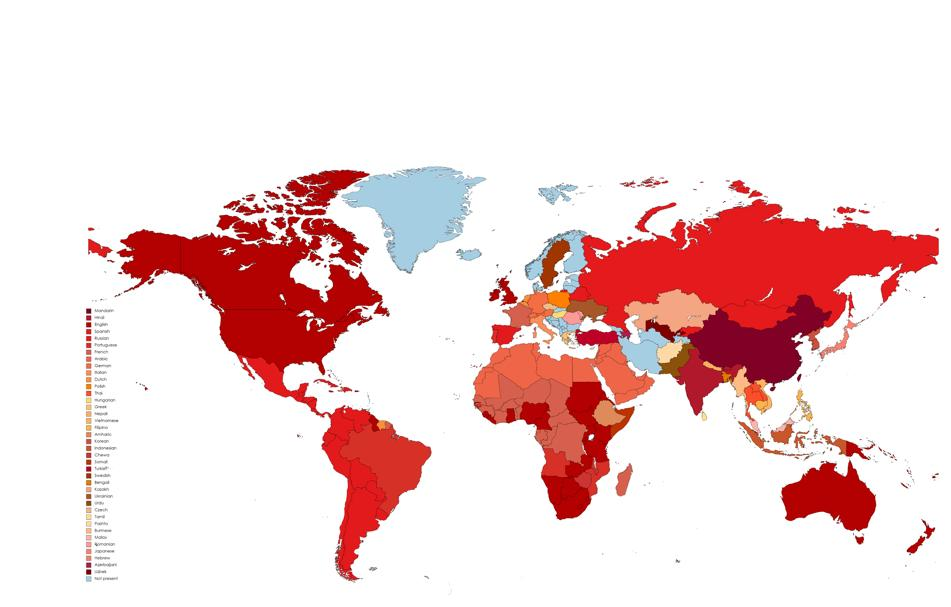
\includegraphics[scale=0.4]{./Images/worldatlas.jpg}

	{\it \footnotesize Figure 6.2: World map to visualize where languages present in the dataset are spoken according to Ethnologue (2022) and WALS (2013), made with mapchart.net} 
\end{center}

\vspace{0.3cm}

\noindent

A closer examination of the blue regions reveals that the Scandinavian, Balkan and Baltic countries predominantly fall into this category. However, it is important to notice that although the language self is not in the dataset, there might be one that is very closely related to it. The languages spoken in Denmark, Norway, Sweden, Finland and Iceland share such close relationships. In cross-border communication, individuals from these regions often just continue using their respective languages (Gooskens, 2007). In the same way, languages in the Balkan region, such as Bosnian and Albanian, share a relatively recent common ancestor with Romanian (Kushniarevich, 2015). This means they still share a lot of vocabulary and grammar. Similarly, the Baltic states exhibit, although there are fewer resemblances, notable similarities with languages such as Hungarian. Hence, these languages are not entirely absent of the data set.

We can do the same observation for the blue countries outside of Europe. Persian, as the official language of Iran, displays strong connections with Kurdish and Pashto and in lesser terms also with Hindi and Bengali (Fortson, 2011). Additionally, due to the high trade during the Mongol empire, Persian has been largely influenced by Arabic and Turkic languages (Perry, 2005). 

Consequently, the only countries in the world for which there lacks any indication of a Proto-Language connection between their national language and our dataset are Greenland and Armenia. Greenlandic, being an Inuit-language, and Armenian, being a language isolate, show too little similarities with other languages. However, the population of these countries would be less than 4 million people, which accounts for less than 0.05% of the global population of 8 billion people. 

\subsection{Weights}

As discussed previously, the source languages of Lojban with more native speakers were deemed more important (Cowan, 1997). Consequently, the scoring system slightly favored languages with higher wights, which seems justifiable as it benefits a larger number of individuals. However, the approach employed by Lojban only focused on the number of native speakers of the given language: Chinese had a larger weight then English. The existence of secondary speakers was completely disregarded. 

The difference between a native and a secondary speaker is the fact that a native speaker the language learns while growing up. On the other hand, a secondary speaker acquires a language later in life, motivated by factors such as work, tourism or recreation. By exclusively utilizing native speakers as a metric for assessing the importance of a language, the developers of Lojban missed the crucial information that the secondary speakers provide. The number of secondary speakers conveys a significant insight into both the language's political influence as its reach. (Saville-Troike, 2017). Besides, it can indicate a lot about vitality and the preservation of the language (Grenoble et al, 2005). Moreover, the secondary speaker count offers us more about the ease of learning the language. All of these are factors that are vital for the language Atlan will be. 

As a result, we contend that secondary speakers should not be forgotten and should even be given relatively more weight than native speakers. As a result, the number of total speakers is calculated by 0.4 times the native speakers and 0.6 times the secondary speakers. Subsequently, these adjusted totals are then normalized to obtain the final weights. This way, the largest language contributes the most to the product. 

\subsection{Lexi and her workings}

\noindent With consensus on the dataset and the weights, the time has come to explain how Lexi generates words from all these languages. Lexi is designed to take an English word as input to start the process. This is very important, because there is only a very select group of unreducible words that need to be generated this way. By taking a meaning as input, we prevent that it generates words we do not want and control the meaning of the new Atlan word. 

This word is then translated into all the languages that make up the trainings set that was just discussed. That way we can find a common pattern in this set of 60 translations. However, it is key to keep in mind that the same letters are often pronounced differently in different words. For example, the sentence ‘the \textit{tear} in my new painting brought a \textit{tear} in my eye’ contains two words that look identical but sound very different. Such heteronyms prove it is not enough to compare words only by their spelling. To investigate how words are pronounced, Lexi now transforms every translation into their IPA format. 

After the constraints of comparison were a bit hardened by this modification, it is possible to soften them now again. That is, because Atlan reduces the number of vowels drastically. This has as a result that certain sounds that are viewed differently in our languages, can only refer to one and the same letter in Atlan. That means that this sound can be viewed as the same in comparison. To achieve this, Lexi can map each IPA sound to the letter it would represent in Atlan, according to the rules discussed in the phonology-chapter. This creates a list with the transcriptions of how the translations would sound in Atlan.  

The only task that is left now is to find the patterns in this set. Since these patterns will form the new Atlan word, it is certain they will always follow one of three patterns: either con-sonant-vowel-consonant (CVC), consonant-vowel (CV) or vowel-consonant (VC). We can look at possible candidates for this pattern by splitting each translation up into every possible combination that follows one of these patterns. This way, Lexi provides a dataset of candidates of the patterns, made up from small parts of natural language translations. 

If we calculate the similarity between every possible pattern and the transcribed translations, we can get the pattern that resembles the words best. However, to simulate the natural way of words generation a bit better, we experiment with some algorithms to make sure we pick the best word, such as evolutionary computing. 

This is a problem-solving technique that uses the principles of natural selection and genetics to find patterns and optimal solutions. Just as in nature, the individual with the highest ‘fitness’ are selected to create new children. Generation after generation this will mean that only the best traits survive, resulting in a solution. By using evolutionary computing, we are trying to simulate a natural way of one word evolving over time, with only the fittest words surviving. In this case, a ‘fit’ individual is on average very similar to all the translations. We calculate the fitness with the previously discussed cosine similarity. 

The fittest individuals create children through a cross-over process. Lexi divides both words in all possible points and then swaps both halves.  For example, if the words \textit{jap} and \textit{tek} are combined, it can recombine into \textit{j-ek} and \textit{t-ap} and similarly \textit{jak} and \textit{tep.} These children, combined with the parents, form again a large pool of possible Atlan words. The best individuals are again selected, and the winners produce the next generation. After 50 generations, the three individuals with the highest scores are selected and crowned as winners. In the end this process gave us the same outcomes as calculating the highest score for all of them. 

In this way, we generated the five best options for every atom of language we needed to exist in Atlan. Another computer program assigned each word one of these options, keeping in mind that some syllables might appear in the list of options for several words. In the end, this leaves us with a lexicon of words that should be easy to learn and remember for almost the entire population.

\section{Semantic atom vocabulary}

\footnotesize
\begingroup
\renewcommand{\numberraise}{-0.15em}
\newcounter{lexi}
\setcounter{lexi}{1}
\newcolumntype{x}[1]{>{\centering\let\newline\\\arraybackslash\hspace{0pt}}p{#1}}
\def\tabb#1{\thelexi.\stepcounter{lexi} #1}
%\hline\end{tabular}%
%\begin{tabular}{|p{0.7\textwidth} | cx{0.2\textwidth}|cx{0.1\textwidth}|}%
%\hline%
\footnotesize
\renewcommand{\corpsgrootte}{12pt}

%	% \begin{tabular}{|l|c|c|}
%	\hline
%	\multicolumn{3}{|c|}{}\\
%	\hline
%		\thelexi.\stepcounter{lexi} & & \\	
%	\hline
%	%\end{tabular}
%}
\begin{center} 
\resizebox{1\textwidth}{!}{%

	%\resizebox{1\textwidth}{!}{
	 \begin{tabular}{|p{0.7\textwidth} | cx{0.2\textwidth}|cx{0.1\textwidth}|}
	%% \begin{tabular}{|l|c|c|}
	\hline
		\multicolumn{3}{|c|}{{\bf MORPHOSYNTAX (V,CV,VC)}}\\
		\hline
		\multicolumn{3}{|c|}{{\bf MOOD MARKERS}}\\ 
	\hline
		\thelexi.\stepcounter{lexi} Exclamative/ 
		imperative/ \newline vocative 
		expletive & O & \Atlano \\	
		\thelexi.\stepcounter{lexi} Interrogative & E & \Atlane \\	
		\thelexi.\stepcounter{lexi} Subjunctive & U & \Atlanu \\	
		\thelexi.\stepcounter{lexi} Stress (prosodic) & A & \Atlana\\	
		\thelexi.\stepcounter{lexi} Relative clause (+ pronoun)& I \newline & \Atlani \\	
	\hline
	%\end{tabular}

	 


%\footnotesize
 
%\resizebox{1\textwidth}{!}{
	% \begin{tabular}{|p{0.6\textwidth} | cx{0.2\textwidth}|cx{0.2\textwidth}|}
	\hline
	\multicolumn{3}{|c|}{\bf LOGICAL OPERATORS}\\
	\hline
		\thelexi.\stepcounter{lexi} Conjunction (and, $\wedge$) & AN & \an \\	
		\thelexi.\stepcounter{lexi} Disjunction (or, $\vee$) & OL & \ol \\	
		\thelexi.\stepcounter{lexi} Conditional (if, $\rightarrow$, {\it ceteris paribus)} & IF & \Atlanif \\	
		\thelexi.\stepcounter{lexi} Conclusion (thus,  therefore $\therefore$) & IS & \is \\	
		\thelexi.\stepcounter{lexi} Negation (not, $\neg $) - sentential/predicate & NE & \Atlanne \\	
		\thelexi.\stepcounter{lexi} All ($\forall$, universal) & AT & \at \\
		\thelexi.\stepcounter{lexi}Some ($\exists$, -few +many) & SO & \so 	\\
		\thelexi.\stepcounter{lexi} Possible ($\diamond$) & PE & \pe \\	
		\thelexi.\stepcounter{lexi} Necessary ($\square$) & SE & \se \\	
	\hline
	%\end{tabular}
	
 


%%\resizebox{1\textwidth}{!}{ \footnotesize
	%% \begin{tabular}{|l|c|c|}
 
	% \begin{tabular}{|p{0.6\textwidth} | cx{0.2\textwidth} | cx{0.2\textwidth}|}
	\hline
		\multicolumn{3}{|c|}{{\bf SYNTACTICAL MARKERS}}\\
	\hline
	\thelexi.\stepcounter{lexi} Accusative (affected thing/person, object, + verb = transitive  & EK & \ek \\	
		\tabb{Genitive (possession,  + verb = to have)} & TA & \ta \\
		\tabb{Dative (receptive,  benifice)} & LO & \lo \\
		\tabb{Instrumental (tool,  method etc.)} & UT & \ut \\
		\tabb{Nominal (noun,  definite object, \newline loanword\idx{loanword}, name (cartouche\idx{cartouche}))} & NA & \na \\
		\tabb{Plural (suffix)  many} & ON & \on \\

		\tabb{Verb  to do $x$} & TU & \tu \\
		\tabb{Predicate (being,  identity, attribute, \newline  adjective (behind noun) adverbs (behind  verb))} & SI & \si \\
		\tabb{Metaphor} & MU & \Atlanmu\\
	\hline
	%\end{tabular}

	 
\hline
\end{tabular}
		}
	\end{center}

\newgeometry{includefoot, bmargin=0pt, tmargin=70pt}
\setlength{\footskip}{-20pt}
		 \begin{center}
\resizebox{1\textwidth}{!}{%
\begin{tabular}{|p{0.7\textwidth} | cx{0.2\textwidth}|cx{0.1\textwidth}|}
\hline


 
	%% \begin{tabular}{|l|c|c|}
	% \begin{tabular}{|p{0.6\textwidth} | cx{0.2\textwidth} | cx{0.2\textwidth}|}
	\hline
		\multicolumn{3}{|c|}{{\bf TENSE/ASPECT MARKERS}}\\
	\hline
		\tabb{Past} & PA & \pa \\
		\tabb{Future} & FE & \fe \\
		\tabb{Beginning} & KA & \ka \\
		\tabb{Perfective} & NI & \Atlanni\\
		\tabb{Progressive} & PO & \po\\
		\tabb{Passive} & PI & \Atlanpi\\
	\hline
	%\end{tabular}

 



 
	%% \begin{tabular}{|l|c|c|}
	% \begin{tabular}{|p{0.6\textwidth} | cx{0.2\textwidth} | cx{0.2\textwidth}|}
	\hline
		\multicolumn{3}{|c|}{{\bf PREPOSITIONS}}\\
	\hline
		\tabb{Coordinate: at  (time/place)} & ET & \et \\
		\tabb{Left (+earth=west)} & LA & \la \\
		\tabb{Right (+earth=east)} & TI & \ti\\
		\tabb{In front (time:before)} & EN & \en\\
		\tabb{Behind (time:after)} & IT & \Atlanit \\
		\tabb{Next to  (right and left)} & KE & \ke\\
		\tabb{Above} & EF & \ef \\
		\tabb{On} & AF & \af\\
		\tabb{Under, below} & OT & \ot\\
		\tabb{Inside  (+time=during)} & IN & \Atlanin \\
		\tabb{Via, through} & LE & \Atlanle\\
		\tabb{Outside} & AP & \ap\\
		\tabb{Surround ing} & AL & \al\\
		\tabb{In between} & MI & \mi\\
		\tabb{Near} & KI & \ki\\
		\tabb{Far} & FA & \fa\\
		\tabb{Horizontal} & IL &\il\\
		\tabb{Vertical} & TE & \te\\
		\tabb{Sagittal} & SA & \sa\\
		\tabb{Direction (of  movement,  combine coordinates x  to y} & LI & \li\\
		\tabb{Range (until, up to)} & TO & \Atlanto\\
		\tabb{Division: per} & EP &\ep\\
		\tabb{Clockwise} & AK & \ak\\
	\hline
	%\end{tabular}

\hline
\end{tabular}
		}
	\end{center}
	\vfill
		 \begin{center}
\resizebox{1\textwidth}{!}{%
\begin{tabular}{|p{0.7\textwidth} | cx{0.2\textwidth}|cx{0.1\textwidth}|}
\hline
 
	%% \begin{tabular}{|l|c|c|}
	% \begin{tabular}{|p{0.6\textwidth} | cx{0.2\textwidth} | cx{0.2\textwidth}|}
	\hline
		\multicolumn{3}{|c|}{{\bf NUMBERS}}\\
	\hline
		\tabb{One} & IP & \thead{\ip  \numbr{1}}\\
		\tabb{Two} & OP & \thead{\op  \numbr{2}}\\
		\tabb{Three} & UP & \thead{\up  \numbr{3}}\\
		\tabb{Four} & IK & \thead{\ik  \numbr{4}}\\
		\tabb{Five} & OK & \thead{\ok  \numbr{5}}\\
		\tabb{Six} &  UK & \thead{\uk  {\numbr{6}}}\\
		\tabb{Seven} &  IM & \thead{\im  \numbr{7}}\\
		\tabb{Eight} & OM & \thead{\om \numbr{8}}\\
		\tabb{Nine} & UM & \thead{\om  \numbr{9}}\\
		\tabb{Ten} & JI & \thead{\ji  \numbr{10}}\\
		\tabb{Eleven} & JO & \thead{\jo  \numbrdd{11}}\\
		\tabb{Twelve} & JU & \thead{\ju  \numbrdd{12}}\\
		\tabb{Hundred (base 10) \newline/144 (base 12)} & NO & \thead{\no}\\
		\tabb{Thousand (base 10) \newline /1728 (base 12)} & NU & \thead{\Atlannu}\\
		\tabb{Exponent} & US & \thead{\us}\\
		\tabb{Ordinal} & OJ & \thead{\oj}\\
	\hline
	%\end{tabular}

 

 
	%% \begin{tabular}{|l|c|c|}
	% \begin{tabular}{|p{0.6\textwidth} | cx{0.2\textwidth} | cx{0.2\textwidth}|}
	\hline
		\multicolumn{3}{|c|}{{\bf SYNTAX-SEMANTIC}}\\
	\hline
		\tabb{Masculine} & MA & \ma\\
		\tabb{Feminine} & FI & \Atlanfi\\
		\tabb{Person} & EJ & \ej\\
		\tabb{Time} & JA & \ja\\
		\tabb{Place} & LU & \lu\\
		\tabb{Demonstrative  (This, that)} & ES & \es\\
\hline
\end{tabular}
		}
	\end{center}
	\vfill

		 \begin{center}
\resizebox{1\textwidth}{!}{%
\begin{tabular}{|p{0.7\textwidth} | cx{0.2\textwidth}|cx{0.1\textwidth}|}
\hline
		\tabb{1st removed: speaker} & AM & \am\\
		\tabb{2nd removed: listener \newline speaking context} & UN & \un\\
		\tabb{3rd removed: beyond context \newline of speaker} & AJ & \aj\\
		\tabb{Part-to-whole relationship} & PU & \pu\\
		\tabb{Final state} & FU & \fu\\
		\tabb{Intention} & UF & \uf\\
		\tabb{Cause, reason (effect = caused, passive)} & KO & \ko\\
		\tabb{Inverse} & EM & \Atlanem\\
		\tabb{Negative} & JE & \je\\
		\tabb{Neutral} & UJ & \uj\\
		\tabb{Positive} & FO & \fo\\
		\tabb{Equative (same as)} & ME &\me\\
		\tabb{Comparative  (more,very)} & MO & \mo\\
		\tabb{Superlative (most)} & AS &\as\\
		\tabb{Contrast (than,  + relative clause  = but)} & KU & \ku\\
		\tabb{Self} & SU & \su\\
		\tabb{Other} & OF &\of\\
		\hline
	%\end{tabular}

	%% \begin{tabular}{|l|c|c|}
	% \begin{tabular}{|p{0.6\textwidth} | cx{0.2\textwidth} | cx{0.2\textwidth}|}
	\hline
		\multicolumn{3}{|c|}{{\bf SEMANTICS - (196-CVC)}}\\
	\hline
		\multicolumn{3}{|c|}{{\bf QUALIA}}\\
	\hline
		\tabb{See} & SIK & \sik\\
		\tabb{Colour\idx{colour}} & KAL & \kal\\
		\tabb{Brightness, light} & LAS & \las\\
		\tabb{Red} & EL & \el\\
		\tabb{Green} & OS & \os\\
		\tabb{Blue} & UL & \ul\\
		\tabb{Hear} & TIN & \tin\\
		\tabb{sound\idx{sound}} & SAN & \san\\
		\tabb{Volume, loudness} & LAT & \lat\\
\hline
\end{tabular}
		}
	\end{center}
	\vfill

		 \begin{center}
\resizebox{1\textwidth}{!}{%
\begin{tabular}{|p{0.7\textwidth} | cx{0.2\textwidth}|cx{0.1\textwidth}|}
\hline
		\tabb{Become, transform} & PIN & \pin\\
		\tabb{Note, pitch} & PIT & \pit\\
		\tabb{Smell\idx{smell}} & SEN & \sen\\
		\tabb{Taste\idx{taste}} & TAS & \tas\\
		\tabb{Sweet} & TIT & \tit\\
		\tabb{Sour} & SAK & \sak\\
		\tabb{Bitter} & KIT & \kit\\
		\tabb{Salty} & SAL & \sal\\
		\tabb{Umami} & MUM & \mum\\
		\tabb{Feeling, affect  (+good=valence \newline +bad =pain)} & SIN & \Atlansin\\
		\tabb{Contact, touch} & TOT & \tot\\
		\tabb{Tension} & JEN & \jen\\
		\tabb{Texture} & TEK & \tek\\
		\tabb{Temperature} & TEP & \tep\\
		\tabb{Balance} & PAN & \pan\\
	\hline
	%\end{tabular}
 

 
%\resizebox{1\textwidth}{!}{
	% \begin{tabular}{|p{0.6\textwidth} | cx{0.2\textwidth}|cx{0.2\textwidth}|}
	\hline
	\multicolumn{3}{|c|}{\bf EMOTIONS}\\
	\hline
	\thelexi.\stepcounter{lexi} Anger & NAK & \nak \\
	\thelexi.\stepcounter{lexi} Anticipation & TIS & \tis \\
	\thelexi.\stepcounter{lexi} Joy & SUS & \sus \\
	\thelexi.\stepcounter{lexi} Trust & FIS & \fis \\
	\thelexi.\stepcounter{lexi} Fear & TEF & \tef \\
	\thelexi.\stepcounter{lexi} Surprise & SAP & \sap \\
	\thelexi.\stepcounter{lexi} Sadness & NUS & \nus \\
	\thelexi.\stepcounter{lexi} Disgust & KAM & \kam \\
	\thelexi.\stepcounter{lexi} Miss & FIP & \fip \\
	\thelexi.\stepcounter{lexi} Love & LOF & \lof \\
	\thelexi.\stepcounter{lexi} Hate & KEF & \kef \\
	\thelexi.\stepcounter{lexi} Regret & LEJ & \lej \\
	\hline
	%\end{tabular}
	
\hline
\end{tabular}
		}
	\end{center}
	\vfill

		 \begin{center}
\resizebox{1\textwidth}{!}{%
\begin{tabular}{|p{0.7\textwidth} | cx{0.2\textwidth}|cx{0.1\textwidth}|}
\hline
 

 
%\resizebox{1\textwidth}{!}{
	% \begin{tabular}{|p{0.6\textwidth} | cx{0.2\textwidth}|cx{0.2\textwidth}|}
	\hline
	\multicolumn{3}{|c|}{\bf CONSCIOUSNESS}\\
	\hline
	\thelexi.\stepcounter{lexi} Consciousness\idx{consciousness}, mind & MAK & \mak \\
	\thelexi.\stepcounter{lexi} Awareness, focus & FEK & \fek \\
	\thelexi.\stepcounter{lexi} Hypnosis & NOS & \nos \\
	\thelexi.\stepcounter{lexi} Dissociation & LIS & \lis \\
	\thelexi.\stepcounter{lexi} Trance, depersonalization & JAS & \jas \\
	\thelexi.\stepcounter{lexi} Sleep & SUL & \sul \\
	\thelexi.\stepcounter{lexi} Hallucination & TAN & \Atlantan \\
	\thelexi.\stepcounter{lexi} Depression & TEJ & \tej \\
	\thelexi.\stepcounter{lexi} Stimulation, excitation \newline(negative = sedation) & JIS & \jis \\
	\thelexi.\stepcounter{lexi} Think, reason, abstract, logic & SIN & \Atlansin \\
	\thelexi.\stepcounter{lexi} Memory, remember & LIM & \Atlanlim \\
	\thelexi.\stepcounter{lexi} Desire, will & FAN & \fan \\
	\thelexi.\stepcounter{lexi} Conscience (moral) & LEN & \len \\
	\thelexi.\stepcounter{lexi} Intuition, instinct & NIT & \nit \\
	\thelexi.\stepcounter{lexi} Imagination, creativity & NIL & \Atlannil \\
	\thelexi.\stepcounter{lexi} Know (+ think = understand) & NEF & \nef \\
	\thelexi.\stepcounter{lexi} Study & SUF & \suf \\
	\hline
	%\end{tabular}
	
 

 
%\resizebox{1\textwidth}{!}{
	% \begin{tabular}{|p{0.6\textwidth} | cx{0.2\textwidth}|cx{0.2\textwidth}|}
	\hline
	\multicolumn{3}{|c|}{\bf EXPRESSION}\\
	\hline
	\thelexi.\stepcounter{lexi} Say, speak & LAN & \lan \\
	\thelexi.\stepcounter{lexi} Greet & MAL & \mal \\
	\thelexi.\stepcounter{lexi} Ask & NUK & \nuk \\
	\thelexi.\stepcounter{lexi} Thank & JEK & \jek \\
	\thelexi.\stepcounter{lexi} Word & SET & \set \\
	\thelexi.\stepcounter{lexi} Book & POK & \pok \\
	\thelexi.\stepcounter{lexi} Read & LET & \Atlanlet \\
	\thelexi.\stepcounter{lexi} Write & LIK & \lik \\
	\thelexi.\stepcounter{lexi} True (yes) & TET & \tet \\
\hline
\end{tabular}
		}
	\end{center}
	\vfill

		 \begin{center}
\resizebox{1\textwidth}{!}{%
\begin{tabular}{|p{0.7\textwidth} | cx{0.2\textwidth}|cx{0.1\textwidth}|}
\hline
	\thelexi.\stepcounter{lexi} Count & NOT & \Atlannot \\
	\thelexi.\stepcounter{lexi} Number & NOM & \nom \\
	\thelexi.\stepcounter{lexi} Measure, amount & MEP & \mep \\
	\thelexi.\stepcounter{lexi} Music (+ voice = sing) & NAN & \nan \\
	\thelexi.\stepcounter{lexi} Voice & FAS & \fas \\
	\thelexi.\stepcounter{lexi} Play & LAJ & \laj \\
	\hline
	%\end{tabular}

 


 
%\resizebox{1\textwidth}{!}{
	% \begin{tabular}{|p{0.6\textwidth} | cx{0.2\textwidth}|cx{0.2\textwidth}|}
	\hline
	\multicolumn{3}{|c|}{\bf GEOMETRY AND TOPOLOGY}\\
	\hline
	\thelexi.\stepcounter{lexi} Big, augmentative & PIK & \pik \\
	\thelexi.\stepcounter{lexi} Long & LAK & \lak \\
	\thelexi.\stepcounter{lexi} Wide & LAM & \lam \\
	\thelexi.\stepcounter{lexi} Thick & TOK & \tok \\
	\thelexi.\stepcounter{lexi} Heavy & PIF & \pif \\
	\thelexi.\stepcounter{lexi} Small, diminutive & SOT & \sot \\
	\thelexi.\stepcounter{lexi} Short & KOT & \kot \\
	\thelexi.\stepcounter{lexi} Narrow & NEJ & \nej \\
	\thelexi.\stepcounter{lexi} Thin & PUT & \Atlanput \\
	\thelexi.\stepcounter{lexi} Sufficient (too, enough) & SEF & \sef \\
	\thelexi.\stepcounter{lexi} Round  & LOK & \lok \\
	\thelexi.\stepcounter{lexi} Flat & FET & \pet \\
	\thelexi.\stepcounter{lexi} Thin & PUT & \Atlanput \\
	\thelexi.\stepcounter{lexi} Straight & SIT & \sit \\
	\thelexi.\stepcounter{lexi} Hole & TOL & \tol \\
	\thelexi.\stepcounter{lexi} Edge & KAP & \kap \\
	\thelexi.\stepcounter{lexi} Surface & SEM & \sem \\
	\thelexi.\stepcounter{lexi} Spatial volume & NET & \net \\
	\thelexi.\stepcounter{lexi} Axis & KEJ & \kej \\
	\thelexi.\stepcounter{lexi} Ball & POP & \pop \\
	\thelexi.\stepcounter{lexi} Line & LUJ & \luj \\
	\hline
	%\end{tabular}
	
\hline
\end{tabular}
		}
	\end{center}
	\vfill

		 \begin{center}
\resizebox{1\textwidth}{!}{%
\begin{tabular}{|p{0.7\textwidth} | cx{0.2\textwidth}|cx{0.1\textwidth}|}
\hline
 


 
%\resizebox{1\textwidth}{!}{
	% \begin{tabular}{|p{0.6\textwidth} | cx{0.2\textwidth}|cx{0.2\textwidth}|}
	\hline
	\multicolumn{3}{|c|}{\bf PEOPLE}\\
	\hline
	\thelexi.\stepcounter{lexi} Young, new & NUJ & \nuj \\
	\thelexi.\stepcounter{lexi} Old & POL & \pol \\
	\thelexi.\stepcounter{lexi} Partner & JAP & \jap \\
	\thelexi.\stepcounter{lexi} Parent (reduplicate to add generation) & PET & \pet \\
	\thelexi.\stepcounter{lexi} Child (daughter, son) & TAT & \tat \\
	\thelexi.\stepcounter{lexi} Sibling & SIP & \sip \\
	\thelexi.\stepcounter{lexi} Acquaintance (friend, enemy) & TEN & \ten \\
	\hline
	%\end{tabular}

 



 
%\resizebox{1\textwidth}{!}{
	% \begin{tabular}{|p{0.6\textwidth} | cx{0.2\textwidth}|cx{0.2\textwidth}|}
	\hline
	\multicolumn{3}{|c|}{\bf FLORA AND FAUNA}\\
	\hline
	\thelexi.\stepcounter{lexi} Nature & NIF & \nif \\
	\thelexi.\stepcounter{lexi} Creature, organism & NIK & \nik \\
	\thelexi.\stepcounter{lexi} Virus & SIF & \sif \\
	\thelexi.\stepcounter{lexi} Bacteria & JIK & \jik \\
	\thelexi.\stepcounter{lexi} Archaea & NUL & \nul \\
	\thelexi.\stepcounter{lexi} Amoeba & PAM & \pam \\
	\thelexi.\stepcounter{lexi} Plant & TUP & \tup \\
	\thelexi.\stepcounter{lexi} Fungus & KON & \kon \\
	\thelexi.\stepcounter{lexi} Animal & NAF & \naf \\
	\thelexi.\stepcounter{lexi} Mammal & MAM & \mam \\
	\thelexi.\stepcounter{lexi} Fish & MIS & \mis \\
	\thelexi.\stepcounter{lexi} Bird & PAJ & \paj \\
	\thelexi.\stepcounter{lexi} Insect & KES & \kes \\
	\thelexi.\stepcounter{lexi} Reptile & LEP & \lep \\
	\thelexi.\stepcounter{lexi} Worm & LEM & \lem \\
	\thelexi.\stepcounter{lexi} Tree (+ substance = wood) & TEL & \tel \\
	\thelexi.\stepcounter{lexi} Eco\idx{Eco, Umberto}system, biome (+ tree = forest) & PIM & \pim \\
	\thelexi.\stepcounter{lexi} Stick, branch & FAP & \fap \\
		\thelexi.\stepcounter{lexi} Fruit$\textsubscript{(+ fungus = mushroom)}$ & FUT & \fut \\
		\thelexi.\stepcounter{lexi} Seed$\textsubscript{(+ fungus = spore, + animal = sperm)}$ & NIP & \nip \\
	\thelexi.\stepcounter{lexi} Leaf & LIF & \lif \\
		\thelexi.\stepcounter{lexi} Root$\textsubscript{(+ fungus = mycelium, + shape = rhizome)}$ & LUT & \lut \\
	\thelexi.\stepcounter{lexi} Flower & FAL & \fal \\
	\thelexi.\stepcounter{lexi} Grass & SOK & \sok \\
	\thelexi.\stepcounter{lexi} Rope & LOS & \los \\
	%\end{tabular}
\hline
\end{tabular}
		}
	\end{center}
\vfill
 

 \begin{center}
\resizebox{1\textwidth}{!}{%
\begin{tabular}{|p{0.7\textwidth} | cx{0.2\textwidth}|cx{0.1\textwidth}|}
\hline


 
	%% \begin{tabular}{|l|c|c|}
% \begin{tabular}{|p{0.6\textwidth} | cx{0.2\textwidth} | cx{0.2\textwidth}|}
\hline
	\multicolumn{3}{|c|}{{\bf ORAL VERBS}}\\
\hline
\tabb{	Consume (+ solid = eat, \newline + liquid = drink)  }
&
KOS 
	
&
\kos 
\\
\tabb{	Bite  }
	
&
JAT 
	
&
\jat 
\\
\tabb{	Suck  }
	
&
SOS 
	
&
\sos 
\\
\tabb{	Spit  }
	
&
TUS &	

\tus 
\\
\tabb{	Vomit, regurgitate  }
	
&
FOT 
	
&
\fot 
\\
\tabb{	Blow  }
	
&
PUL 
	
&
\pul 
\\
\tabb{	Breathe (+ organ = lung, \newline + smoke = to smoke something)  }
	
&
LUS 
	
&
\lus 
\\
\tabb{	Laugh (humor)  }
	
&
LAF 
	
&
\laf 
\\
\tabb{	Cry  }
	
&
KAJ 
	
&
\kaj 
\\
\tabb{   Shout  }
	
&
NOJ 
	
&
\noj 
\\
\hline
%\end{tabular}

%%
 
%\resizebox{1\textwidth}{!}{
	% \begin{tabular}{|p{0.6\textwidth} | cx{0.2\textwidth}|cx{0.2\textwidth}|}
	\hline
	\multicolumn{3}{|c|}{\bf ANATOMY}\\
	\hline
	\thelexi.\stepcounter{lexi} Skin (+ tree = bark, + material = leather) & POS & \pos \\
	\thelexi.\stepcounter{lexi} Meat, flesh, muscle & MAF & \maf \\
	\thelexi.\stepcounter{lexi} Blood & KAT & \kat \\
	\thelexi.\stepcounter{lexi} Milk (+ organ = breast) & TIL & \til \\
	\thelexi.\stepcounter{lexi} Slime, mucus (+ mouth = saliva,\newline + nose = snot) & LIL & \lil \\
	\thelexi.\stepcounter{lexi} Bone & KOP & \kop \\
	\thelexi.\stepcounter{lexi} Fat & FAT & \fat \\
	\thelexi.\stepcounter{lexi} Egg & TAJ & \taj \\
	\thelexi.\stepcounter{lexi} Horn & PON & \pon \\
	\thelexi.\stepcounter{lexi} Tail & KET & \ket \\
\hline
\end{tabular}
		}
	\vfill
	\end{center}

		 \begin{center}
\resizebox{1\textwidth}{!}{%
\begin{tabular}{|p{0.7\textwidth} | cx{0.2\textwidth}|cx{0.1\textwidth}|}
\hline
	\thelexi.\stepcounter{lexi} Feather & PEF & \pef \\
	\thelexi.\stepcounter{lexi} Hair & PEL & \pel \\
	\thelexi.\stepcounter{lexi} Head & SAT & \sat \\
	\thelexi.\stepcounter{lexi} Face & LES & \les \\
	\thelexi.\stepcounter{lexi} Organ (+ hear = ear, + see = eye,\newline + smell\idx{smell} = nose, + taste\idx{taste} = tongue) & NOK & \nok \\
	\thelexi.\stepcounter{lexi} Tissue & JUS & \jus \\
	\thelexi.\stepcounter{lexi} Cell & SEL & \sel \\
	\thelexi.\stepcounter{lexi} Mouth & MUT & \mut \\
	\thelexi.\stepcounter{lexi} Lips (+ touch = kiss) & LIP & \lip \\
	\thelexi.\stepcounter{lexi} Cheeks & KIS & \kis \\
	\thelexi.\stepcounter{lexi} Tooth & TUN & \tun \\
	%\end{tabular}

 


 
%\resizebox{1\textwidth}{!}{
	% \begin{tabular}{|p{0.6\textwidth} | cx{0.2\textwidth}|cx{0.2\textwidth}|}
	\thelexi.\stepcounter{lexi} Nail & NEK & \nek \\
	\thelexi.\stepcounter{lexi} Foot & PAF & \paf \\
	\thelexi.\stepcounter{lexi} Leg & LUK & \luk \\
	\thelexi.\stepcounter{lexi} Joint (+ leg = knee, \newline+ arm = elbow, + line = angle) & TUJ & \tuj \\
	\thelexi.\stepcounter{lexi} Hand & JAM & \jam \\
	\thelexi.\stepcounter{lexi} Finger (+ foot = toe) & FEN & \fen \\
	\thelexi.\stepcounter{lexi} Arm & MAP & \map \\
	\thelexi.\stepcounter{lexi} Wing & KIN & \kin \\
	\thelexi.\stepcounter{lexi} Belly (+ inside = guts) & PEP & \pep \\
	\thelexi.\stepcounter{lexi} Neck & KEN & \ken \\
	\thelexi.\stepcounter{lexi} Shoulders & TOP & \Atlantop \\
	\thelexi.\stepcounter{lexi} Back & PUK & \puk \\
	\thelexi.\stepcounter{lexi} Chest & SOP & \sop \\
	\thelexi.\stepcounter{lexi} Heart & JOT & \Atlanjot \\
	\thelexi.\stepcounter{lexi} Liver & KAF & \kaf \\
	\thelexi.\stepcounter{lexi} Brain & NEL & \nel \\
	\thelexi.\stepcounter{lexi} Genital & NEN & \nen \\
	\thelexi.\stepcounter{lexi} Waste\idx{taste} (+ solid = faeces, + liquid = urine) & FES & \fes \\
	%\end{tabular}
\hline
\end{tabular}
		}
	\end{center}

		 \begin{center}
\resizebox{1\textwidth}{!}{%
\begin{tabular}{|p{0.7\textwidth} | cx{0.2\textwidth}|cx{0.1\textwidth}|}
\hline

 

 
%\resizebox{1\textwidth}{!}{
	% \begin{tabular}{|p{0.6\textwidth} | cx{0.2\textwidth} | cx{0.2\textwidth}|}
	\hline
		\multicolumn{3}{|c|}{{\bf LIFE AND DEATH}}\\
	\hline
	\tabb{	Intercourse, sex }
	
&
SEK 
	
&
\sek 
\\
\tabb{	Birth (+ active = to birth, \newline + passive = to be born) }
	
&
PES 
	
&
\pes 
\\
\tabb{	Grow }
	
&
KEP 
	
&
\kep 
\\
\tabb{	Life }
	
&
FIN 
	
&
\fin 
\\
\tabb{	Disease }
	
&
TIM 
	
&
\tim 
\\
\tabb{	Death }
	
&
MOT 
	
&
\mot 
\\
\tabb{	Kill }
	
&
KIL 
	
&
\kil 
\\
\tabb{	Fight }
	
&
FAJ 
	
&
\faj 
\\
\tabb{	Hunt }
	
&
JAF 
	
&
\jaf 		
\\
	\hline
	%\end{tabular}

	 




 

% \begin{tabular}{|p{0.6\textwidth} | cx{0.2\textwidth} | cx{0.2\textwidth}|}
\hline
\multicolumn{3}{|c|}{{\bf MOVEMENT}}\\
\hline
\tabb{	Hit } &
	

MAT& 
	

\mat\\ 

\tabb{	Cut } &
	

KUT& 
	

\kut\\ 

\tabb{	Split } &
	

TIP & 
	

\tip\\ 

\tabb{	Stab } &
	

SUT & 
	

\sut\\ 

\tabb{	Scratch } &
	

SEJ & 
	

\sej\\ 

\tabb{	Turn } &
	

TON & 
	

\ton\\ 

\tabb{	Move, go } &
	

MEF & 
	

\mef\\ 

\tabb{	Dig } &
	

KIK & 
	

\kik\\ 

\tabb{	Swim } &
	

NAS & 
	

\nas\\ 

\tabb{	Fly } &
	

FUL & 
	

\ful\\ 
\hline
\end{tabular}
		}
	\end{center}
	\vfill

		 \begin{center}
\resizebox{1\textwidth}{!}{%
\begin{tabular}{|p{0.7\textwidth} | cx{0.2\textwidth}|cx{0.1\textwidth}|}
\hline

\tabb{	Walk } &
	

TOM & 
	

\tom\\ 

\tabb{	Come } &
	

KOM & 
	

\kom\\ 
\tabb{	Lie } &
	

LOM & 
	

\lom\\ 

\tabb{	Stand } &
	

TUF & 
	

\tuf\\ 

\tabb{	Sit } &
	

SUP & 
	

\Atlansup\\ 

	\tabb{Fall (+ transitive = drop, \newline + water = sink)}  &
	

KOL & 
	

\kol\\ 

\tabb{	Happen, occur (+ transitive = do) } &
	

NES & 
	

\nes\\ 

\tabb{	Steer (a vehicle) } &
	

JIL & 
	

\jil\\ 

\tabb{Jump} & 
	

MOS & 
	

\mos\\ 

\tabb{Block} & 
	

FOK & 
	

\fok\\ 
\hline
%\end{tabular}
 

 
%\resizebox{1\textwidth}{!}{
% \begin{tabular}{|p{0.6\textwidth} | cx{0.2\textwidth} | cx{0.2\textwidth}|}
\hline
\multicolumn{3}{|c|}{{\bf HANDLING OBJECTS}}\\
\hline
\tabb{	Give (+ passive = receive) } &
	

KIF & 
	

\kif\\ 

\tabb{	Hold } &
	

LEL & 
	

\lel \\ 

\tabb{	Squeeze } &
	

JIP & 
	

\jip\\ 

\tabb{	Rub } &
	

LOP & 
	

\lop\\ 

\tabb{	Wash, clean } &
	

SAS & 
	

\sas\\ 

\tabb{	Wipe } &
	

TAP & 
	

\tap\\ 

\tabb{	Pull } &
	

JAL & 
	

\jal\\ 

\tabb{	Push } &
	

PUS & 
	

\pus\\ 

\tabb{	Throw } &
	

NOL & 
	

\nol\\ 

\tabb{	Tie } &
	

TAL & 
	

\tal\\ 

\tabb{	Sew } &
	

SES & 
	

\ses\\ 

\tabb{	Shake, vibrate } &
	

JAK & 
	

\jak\\ 

\tabb{	Pick, take } &
	

NEP & 
	

\nep\\ 

\tabb{	Make, create } &
	

MEN & 
	

\men\\ 
\tabb{ Find} &
	

FUN & 
	

\fun\\ 

\tabb{Meet} &
	

MIF & 
	

\mif\\ 

\tabb{Hang} &
	

NUN & 
	

\nun\\ 

\tabb{Kick} &
	

KUP & 
	

\kup\\ 

\tabb{ Exchange } &
	

JEM & 
	

\jem\\ 

\tabb{ Sell } &
MEM & 

\mem\\ 
	


\hline
\end{tabular}
		}
	\end{center}

		 \begin{center}
\resizebox{1\textwidth}{!}{%
\begin{tabular}{|p{0.7\textwidth} | cx{0.2\textwidth}|cx{0.1\textwidth}|}
\hline
\tabb{ Steal } &
JOF & 
\jof\\ 

\tabb{ Attach } &
	

NUF & 
	

\mif\\ 

\tabb{  Replace } &
	

LUP & 
	

\lup\\ 

\tabb{  Gather } &
	

SOJ & 
	

\soj\\ 

\tabb{ Search } &
	

SOF & 
	

\sof\\ 

\tabb{ Wait } &
	

JES & 
	

\jes\\ 

\tabb{ Change } &
	

MEJ & 
	

\mej\\ 

\tabb{ To stick, stay } &
	

PUJ & 
	

\puj\\ 
%\hline
%%\end{tabular}

% 
%
% 
%%\resizebox{1\textwidth}{!}{
%% \begin{tabular}{|p{0.6\textwidth} | cx{0.2\textwidth} | cx{0.2\textwidth}|}
%\hline
%	\multicolumn{3}{|c|}{{\bf HANDLING OBJECTS (Continued) }}\\ 
%\hline
%
\tabb{ Open } &
	

KOF & 
	

\kof\\ 

\tabb{ Control } &
	

JON & 
	

\jon\\ 

\tabb{ Order}  &
	

MOM & 
	

\mom\\ 

\tabb{ Allow } &
	

MUL & 
	

\mul\\ 

\tabb{ Try } &
	

MOK & 
	

\mok\\ 


\hline
%\end{tabular}		%\tabb{} &  & \thead{}}\\

 



 
%\resizebox{1\textwidth}{!}{
% \begin{tabular}{|p{0.6\textwidth} | cx{0.2\textwidth} | cx{0.2\textwidth}|}
\hline
\multicolumn{3}{|c|}{{\bf SUBSTANCE}}\\
\hline
\tabb{	Matter, substance, material } &
	

MAJ &
	

\maj \\ 

\tabb{ Thing } &
	

MUS &
	

\mus \\ 

\tabb{	Weight, heavy } &
	

NEM &
	

\nem \\ 

\tabb{	Water } &
	

NAT &
	

\nat \\ 

\tabb{	Liquid } &
	

JIT &
	

\jit \\ 

\tabb{	Flow } &
	

FEL &
	

\fel \\ 

	\tabb{Wave} &
	

PEJ &
	

\pej \\ 

\tabb{	Float } &
	

TAF &
	

\taf \\ 

\tabb{	Freeze } &
	

LIN &
	

\lin \\ 

\tabb{	Ice} &
	

PIS &
	

\pis \\ 

\tabb{	Snow } &
	

SEP &
	

\sep \\ 

\tabb{	Swell } &
	

SUN &
	

\sun \\ 

\tabb{	Rain } &
	

JUL &
	

\jul \\ 

\tabb{	Soil } &
	

SOL &
	

\sol \\ 

\tabb{	Solid } &
	

TOJ &
	

\toj \\ 

\tabb{	Stone\idx{tone} } &
	

JET &
	

\jet \\ 

\tabb{	Sand} &
	

SAJ &
	

\saj \\ 
\tabb{	Dust} &
	

TUL &
	

\tul \\ 
\hline
\end{tabular}
		}
	\end{center}
\vfill

\vspace{-1cm}
\begin{center}
\resizebox{1\textwidth}{!}{%
\begin{tabular}{|p{0.7\textwidth} | cx{0.2\textwidth}|cx{0.1\textwidth}|}
\hline

\tabb{	Air, wind } &
	

KE &
	

\ke \\ 

\tabb{	Gas} &
	

KA &
	

\ka \\ 

\tabb{	Sky } &
	

SO &
	

\so \\ 

\tabb{	Cloud } &
	

NA &
	

\na \\ 

\tabb{	Fog } &
	

TU &
	

\tu \\ 
\tabb{	Fire } &
	

FA &
	

\fa \\ 

\tabb{	Burn } &
	

PE &
	

\pe \\ 

\tabb{	Smoke } &
	

TU &
	

\tu \\ 

\tabb{	Ash } &
	

KA &
	

\ka \\ 

\tabb{	Metal } &
	

MI &
	

\mi \\ 

\tabb{	Glass } &
	

KU &
	

\ku \\ 

\tabb{	Paper} &
	

PE &
	

\pe \\ 

\tabb{	Textile } &
	

TI &
	

\ti \\ 

\tabb{	Rubber } &
	

LA &
	

\la \\ 

\tabb{	Foam } &
	

MO &
	

\mo \\ 

\tabb{	Petrol-based substance (+ solid = plastic, + liquid = oil) } &
	

PA &
	

\pa \\ 

\tabb{	Molecule } &
	

ME &
	

\me \\ 

\tabb{	Atom (+ number = chemical element)} &
	

TA &
	

\ta \\ 

\tabb{	Particle } &
	

KI &
	

\ki \\ 

\tabb{ Explode } &
	

FO &
	

\fo \\ 

\tabb{ Shrink } &
	

FU &
	

\fu \\ 

\tabb{ Pure } &
	

PU &
	

\pu \\ 

\hline
%\end{tabular}

 
 
%\resizebox{1\textwidth}{!}{
% \begin{tabular}{|p{0.6\textwidth} | cx{0.2\textwidth} | cx{0.2\textwidth}|}
\hline
\multicolumn{3}{|c|}{{\bf GEOLOGY AND ASTRONOMY}}\\
\hline
\tabb{	Sun } &
	

SON  &
	

\son  \\

\tabb{	Star } &
	

SIS  &
	

\sis  \\

\tabb{	Planet } &
	

PAL  &
	

\pal  \\

\tabb{	Earth planet } &
	

TEM  &
	

\tem  \\

\tabb{	Night } &
	

NAJ  &
	

\naj  \\

\tabb{	Day } &
	

JAN  &
	

\jan  \\

\tabb{	Week } &
	

MIK  &
	

\mik  \\

\tabb{	Year } &
	

JIN  &
	

\jin  \\
\hline
\end{tabular}
		}
	\end{center}
	\vspace{3cm}
\clearpage
\vfill\vfill
		 \begin{center}
\resizebox{1\textwidth}{!}{%
\begin{tabular}{|p{0.7\textwidth} | cx{0.2\textwidth}|cx{0.1\textwidth}|}
\hline
\tabb{	Orbital system (+ sun = solar system, \newline + star = galaxy) } &
	

LOT  &
	

\lot  \\

\tabb{	Moon (+ time = month) } &
	

MUN  &
	

\mun  \\

\tabb{	Mountain (+ sand = dune) } &
	

MAN  &
	

\man  \\

\tabb{Top, peak }   &
	

FON  &
	

\fon  \\

\tabb{	Plain } &
	

PAS  &
	

\pas  \\

\tabb{	Ground  } &
	

NAM  &
	

\nam  \\

\tabb{	Country } &
	

MES  &
	

\mes  \\

\tabb{	Continent } &
	

KUN  &
	

\kun  \\

\tabb{	Island } &
	

PIL  &
	

\pil  \\

\tabb{	Road  } &
	

LOL  &
	

\lol  \\

\tabb{	River } &
	

LEF  &
	

\lef  \\

\tabb{	Lake } &
	

LEK  &
	

\lek  \\

\tabb{	Sea } &
	

SAM  &
	

\sam \\
\hline
%\end{tabular}

 




 
%\resizebox{1\textwidth}{!}{
% \begin{tabular}{| p{0.6\textwidth} | cx{0.2\textwidth}| cx{0.2\textwidth}|}
\hline
\multicolumn{3}{|c|}{{\bf QUALITIES}}\\
\hline
\tabb{Origin } &
JOL &
\jol  \\

\tabb{	Full } &

MOL  &

\mol  \\

\tabb{	Good } &

POT  &

\pot  \\

\tabb{	Bad } &

PAK  &
\pak  \\

\tabb{	Rotten } &

LAL  &

\lal  \\

\tabb{	Dirty } &

JUT  &

\jut  \\

\tabb{	Sharp (+ negation = dull) } &

TAK  &

\tak  \\

\tabb{	Smooth, soft } &
SAF  &

\saf  \\

\tabb{	Hard, tough } &

TOF  &

\tof  \\

\tabb{	Difficult } &
TIF  &

\tif  \\

\tabb{	Wet } &

SIL  &

\sil  \\

\tabb{	Dry } &

SUK  &

\suk  \\

\tabb{	Correct } &

KEK  &

\kek  \\

\tabb{	Beautiful  } &

LIT  &

\lit  \\

\tabb{	Ugly } &

KUL  &

\kul  \\

\tabb{	Strong } &

TUT  &

\tut  \\

\tabb{	Weak } &

FIK  &

\fik  \\
\hline
\end{tabular}
		}
	\end{center}
\vfill
		 \begin{center}
\resizebox{1\textwidth}{!}{%
\begin{tabular}{|p{0.7\textwidth} | cx{0.2\textwidth}|cx{0.1\textwidth}|}
\hline

\tabb{      Quick } &

KIM  &

\kim  \\

\tabb{      Slow } &

NIM  &

\nim  \\

\tabb{      High } &

JEJ  &

\jek  \\

\tabb{      Low } &

MEK  &

\mek  \\

\tabb{      Real } &

LEJ  &

\lej  \\

\tabb{      Last } &

LUM  &

\lum  \\

\tabb{     Previous } &

POP  &

\pop  \\

\tabb{     Relevant } &

FEJ  &

\fej  \\

\tabb{      Silly } &

NUP  &

\nup  \\

\tabb{      Extra } &

JEF  &

\jef  \\

\hline
%\end{tabular}

 



 
%\resizebox{1\textwidth}{!}{
% \begin{tabular}{|p{0.6\textwidth} | cx{0.2\textwidth} | cx{0.2\textwidth}|}
\hline
\multicolumn{3}{|c|}{{\bf CULTURE}}\\
\hline
\tabb	Home, domestic  &
	

KEM  &
	

\kem  \\

\tabb	School  &
	

SUJ  &
	

\suj  \\

\tabb	Town, city, village  &
	

TOS  &
	

\tos  \\

\tabb	Culture, customs  &
	

KUK  &
	

\kuk  \\

\tabb	Job, profession  &
	

KAN  &
	

\kan  \\

\tabb	Money  &
	

MON  &
	

\mon  \\

\tabb	Politics  &
	

NIN  &
	

\nin  \\

\tabb{    Tradition } &
	

NOP  &
	

\nop  \\

\tabb	Individual  &
	

FIT  &
	

\fit  \\

\tabb	Community, collective  &
	

SUM  &
	

\Atlansum  \\

\tabb{    Group } &
	

KOK  &
	

\kok  \\

\tabb	Science  &
	

NIS  &
	

\nis  \\

\tabb	Law  &
	

LON  &
	

\lon  \\

\tabb	King, chief, president  &
	

TES  &
	

\tes  \\

\tabb	Medicine  &
	

MET  &
	

\met  \\

\tabb	Machine  &
	

MAS  &
	

\mas  \\

\tabb	Vehicle   &
	

FIL  &
	

\fil  \\

\tabb	Wheel  &
	

MIL  &
	

\mil  \\

\tabb{  Building block } &
	

FUK  &
	

\fuk  \\

\tabb{    Layer } &
	

FEM  &
	

\fem  \\

\tabb{   Projectile } &
	

PEM  &
	

\pem  \\

\tabb	Pipe   &
	

PAP  &
	

\pap  \\

\tabb	Wire  &
	

FAF  &
	

\faf  \\
\hline
\end{tabular}
		}
	\end{center}

\newgeometry{includefoot, bmargin=0pt, tmargin=70pt}    
\setlength{\footskip}{-20pt}


		 \begin{center}
\resizebox{1\textwidth}{!}{%
\begin{tabular}{|p{0.7\textwidth} | cx{0.2\textwidth}|cx{0.1\textwidth}|}
\hline

\tabb	Engine  &
	

NUT  &
	

\nut  \\

\tabb	Electricity, energy  &
	

MIN  &
	

\Atlanmin  \\

\tabb	Computer  &
	

KUM  &
	

\kum  \\

\tabb{ System  } &
	

JIM  &
	

\jim  \\
%\hline
%%\end{tabular}
%}
% 
%
% 
%%\resizebox{1\textwidth}{!}{
%% \begin{tabular}{|p{0.6\textwidth} | cx{0.2\textwidth} | cx{0.2\textwidth}|}
%\hline
%	\multicolumn{3}{|c|}{{\bf CULTURE (Continued)}}\\
%\hline
%

\tabb{Building}  &
	

NAP  &
	

\nap  \\

\tabb{ Wall } &
	

MUK  &
	

\muk  \\

\tabb{ Door } &
	

MIP  &
	

\mip  \\

\tabb{ Container } &
	

NON  &
	

\non  \\

\tabb	God  &
	

JEL  &
	

\jel  \\

\tabb{    Peace } &
	

PUN  &
	

\pun  \\

\tabb{   Problem, Conflict } &
	

POM  &
	

\pom  \\

\tabb{   Mistake } &
	

KUF  &
	

\kuf  \\

\tabb{  Destruction } &
	

JUN  &
	

\jun  \\

\tabb	Picture, image  &
	

SIM  &
	

\Atlansim \\

\tabb{   Symbol } &
	

MIM  &
	

\mim  \\

\tabb	Family  &
	

FAM  &
	

\Atlanfam  \\

\tabb	Story  &
	

JOS  &
	

\jos  \\

\tabb{      Garbage } &
	

LUL  &
	

\lul  \\

\tabb{ Clothes } &
	

KEF  &
	

\kef  \\

\tabb{   Furniture } &
	

MUP  &
	

\mup  \\

\tabb{    Symmetry } &
	

FIM  &
	

\fim  \\

\tabb{   Reflection } &
	

FEP  &
	

\fep  \\

\tabb{  Complexity } &
	

KOJ  &
	

\koj  \\

\tabb{\footnotemark Success } &

	

JUK  &
	

\juk  \\

\hline
\end{tabular}
}
\end{center} 

$^1${\normalsize \noindent Not all syllable\idx{syllable}s were used, since we have 490 options in total, there are 42 additional syllables which weren't used and can be used when additional words are added when expanding the language.}

A searchable online lexicon can be found on https://www.Atlanial.com.

\endgroup
\vfill
\restoregeometry
\setlength{\footskip}{60pt}

\normalsize
\restorecorps

\section{Protocol for translation}

Atlan’s lexicon is composed by adding together different semantic atoms (see: oligosynthesis). Meaning is specified by following the principle of a “semantic lens” which “zooms in” with every atom that is added, reducing the possible meanings of a word to a more defined meaning. The order in which atoms are added is structured hierarchically. The first atom specifies the most basic classification of the intended word, to which other atoms are appended which incrementally specify the exact definition. Two combinations of the same atoms that are ordered in different ways (e.g. AB and BA) will thus have different definitions. For example: 

\begin{itemize}
\item[] Bird + house = a pet bird (a bird pertaining to the domestic) 

\item[] House + bird = a bird’s nest (the house of a bird) 

\item[]  

\item[] Flower + smell = a fragrant flower (a flower which smells) 

\item[] Smell + flower = a floral scent (the smell of a flower) 

\item[]  

\item[] Sing + community = to sing in a choir (to sing communally) 

\item[] Community + sing = a choir (a community of singers / singing) 
\end{itemize}

\noindent 

Morphosyntactic atoms can be recognised by the fact that they contain one one consonant and syllable (not CVC). These are always put in front of the main semantic atom, again following the principle of hierarchy, and taking into account the scope of each atom. Any atom only determines the scope of the atoms that come after it, not the ones that come before it. For example:

\begin{itemize}
\item[] Passive + give = to receive X (to be given X: to receive a gift = to be given a gift) 

 

\item [] Passive + give + (dative) = to be given to X (the gift was given given to them) 

 

\item []Predicate + not + life = (to be) inanimate 

 

\item [] Not + predicate + life = not (to be) alive 

\end{itemize}

\noindent Finally, the plural marker comes at the very end of a word. The general order for compound words it thus:  

\begin{center}
morphosyntactic markers - main semantic root - specifying semantic atoms – plural
\end{center}

It must be noted that translations are open to individual and cultural interpretation. As long as the hierarchical structure of word formation is obeyed, different approaches to specifying the same word are possible. For example: 



\begin{itemize}
\item [] Fish + fly = flying fish (a fish which flies) 

\item[] Fish + wing = flying fish (a fish with wings) 

 

\item[] Vehicle + sea = boat (a vehicle for the sea) 

\item[] Vehicle + float = boat (a vehicle which floats)
\end{itemize}

\noindent Because of their sheer quantity and diversity, words for specific human artifacts can sometimes be more challenging to synthesize. Phonetically approximated loanwords can be employed when referring to specific cultural artefacts or concepts (see chapter 3.7), marked by the name particle NA, together with a cartouche in written language. 

Expletives, better known as swear words, can be made by adding the prefix ´O´ \Atlano to mark the exclamatory nature, followed by a literal translation of the word, which will thus be culture dependent (e.g.: ´shit´ = O.FES.TOJ \Atlano \fes \toj). 

\section{Jargon translation}


Atlan’s established lexicon will not be enough to cover the large quantity of topic/discipline-specific jargon within human language. Specialists within their respective fields could formalize nomenclature systems which could then be adopted by their respective intellectual communities as the standard for communicating about their subject matters in Atlan as an auxlang. This could be a natural evolution within the arts and sciences away from obsolete and culturally imposed greco-latin terminology of the European academic tradition, as well as serving as an opportunity for scientists who often complain about illogical and arbitrary terminology within their subject to collectively design a rigorous reform towards more logical and useful words in a more neutral lingua franca.  

We cannot dictate in this context how each discipline will end up standardizing their terminology in Atlan, but we could suggest taking inspiration from original etymologies and nomenclatures already in place as standardized systems. We will not further expound on how this should be done here, since this is beyond our own expertise, and almost impossible to cover comprehensively.







